\documentclass{article}

% if you need to pass options to natbib, use, e.g.:
\PassOptionsToPackage{numbers}{natbib}
% before loading nips_2016
%
% to avoid loading the natbib package, add option nonatbib:
% \usepackage[nonatbib]{nips_2016}

\usepackage[final]{nips_2016} % produce camera-ready copy
% to compile a camera-ready version, add the [final] option, e.g.:
% \usepackage[final]{nips_2016}

\usepackage[utf8]{inputenc} % allow utf-8 input
\usepackage[T1]{fontenc}    % use 8-bit T1 fonts
\usepackage{hyperref}       % hyperlinks
\usepackage{url}            % simple URL typesetting
\usepackage{booktabs}       % professional-quality tables
\usepackage{amsfonts}       % blackboard math symbols
\usepackage{nicefrac}       % compact symbols for 1/2, etc.
\usepackage{microtype}      % microtypography
\usepackage{blindtext}
\usepackage{amsmath}
\usepackage{graphicx}
\usepackage{float}
\usepackage{tabularx}
\usepackage{xcolor,colortbl}
\usepackage{caption}

\title{Sentiment Classification from Movie Reviews}

\author{
  Dainius Saltenis\\
  s2124779\\
  \texttt{D.Saltenis@sms.ed.ac.uk} \\
  %% examples of more authors
  \And
  Oliver Aarnikoivu\\
  s2125219\\
  \texttt{O.Aarnikoivu@sms.ed.ac.uk} \\
}

\begin{document}

\maketitle

\begin{abstract}
Sentiment classification is one of the most practical and useful text classification problems, however, to accurately detect sentiment from text is extremely challenging. While previous research has placed focus on classifying sentiment at the sentence-level using primarily supervised approaches, we apply both supervised and unsupervised machine learning methods to fine-grained \emph{phrase}-level sentiment analysis, using the Stanford Sentiment Treebank (SST) dataset. With regards to supervised classification, we find that making use of feature engineering is important to consider for improving classification performance. We show that reducing the dimensionality of feature vectors using Linear Discriminant Analysis (LDA) is highly effective in preserving class separability in lower dimensional space. Regarding unsupervised learning, we show that by applying Agglomerative Clustering to embeddings produced by a fully-connected auto-encoder, we're able to uncover some of the underlying hidden structure of phrases better than other cluster-based techniques.  
\end{abstract}

\section{Introduction}

Sentiment classification is arguably one of the most practical and useful text classification problems, however, to accurately detect sentiment from text is extremely challenging. This is because there are a variety of complexities associated with language, such as sarcasm, ambiguity, plurality, punctuation, and other imprecise characteristics. Due to these challenges, much of the existing research has been fixated on treating the task of sentiment classification as a binary problem, i.e. a text can either be "positive" or "negative". Additionally, although a variety of datasets with document labels are available \cite{maas-etal-2011-learning}, \cite{article}, there is still a need to better capture sentiment from shorter text, such as Twitter, Facebook and YouTube \cite{socher-etal-2013-recursive}. Moreover, many of the existing approaches have neglected the use of unsupervised methods. Unsupervised sentiment analysis could be useful when there isn't a lot of labeled data available, and when we are unsure about the underlying structure of the data \cite{Hastie2009}. 

\subsection{Objective}

In this report we explore both supervised and unsupervised methods on a dataset of movie phrases (groups of words that act as a part of speech) that have been labeled with a degree of sentiment on a 5-point scale from positive to negative, also known as \emph{fine-grained sentiment analysis}. In the supervised approach, the objective is to predict the sentiment of a given phrase into one of the 5-point scale labels, whereas in the unsupervised approach the objective is to uncover the underlying structure of the data using cluster-based methods. We begin with an extensive exploratory data analysis in order to discover meaningful information about the dataset. We use feature engineering and extraction to discriminate positive, neutral and negative sentiment. We assess a variety of classifiers using a two-times hold out approach. Finally, we experiment on using unsupervised dimensionality reduction and clustering algorithms to classify sentiment without having sentiment labels for training.

\subsection{Relevant Background and Previous Work}

Previous research has been widely conducted using the SST dataset,\footnote{\url{https://nlp.stanford.edu/sentiment/index.html}} where evaluation of models is mostly applied on fine-grained sentiment classification, and binary sentiment classification. Other popular sentiment classification datasets are also present, such as the IMDb movie review dataset \cite{maas-etal-2011-learning} or subsets of large Amazon reviews dataset \cite{he2016ups}. For the task related to this report (fine-grained sentiment classification), it's important to note that previous research is primarily applied at the sentence level as opposed to phrases, with the exception of \cite{yin-etal-2020-sentibert}. Nonetheless, we believe that methods applied at both the sentence and phrase level are highly interchangeable. Therefore, this section focuses on existing research with regards to sentence-level sentiment classification. However, do note that the results achieved by the following authors are not representative of the results attained in this report. 

Prior to the deep learning era, previous machine learning approaches required extensive feature engineering in order to perform well on sentiment classification. To discriminate categories, it was crucial to incorporate domain-knowledge, taking advantage of additional features such as word frequency, part of speech tags, term positions and negation \cite{DBLP:journals/corr/KhardeS16}. However, with the advent of deep learning, the need to include additional features has been diminished. Today, current state-of-the-art approaches in sentiment classification are dominated by highly paramaterised, and novel deep learning architectures which largely build on the Transformer \cite{DBLP:journals/corr/VaswaniSPUJGKP17} and its variants, such as BERT (Bidirectional Encoder Representations from Transformers) \cite{DBLP:journals/corr/abs-1810-04805}. 

The current state-of-the-art for fine-grained sentiment classification is achieved by the authors \cite{sun2020self}, who report an accuracy of 59.1. The authors apply the RoBERTa transformer architecture and offer a novel layer to aggregate output information of model output steps to enhance the performance. Previous state-of-the-art exploited a more outdated and differing approach by using sequential models. Brahma \cite{brahma2018improved} reports an accuracy of 56.2 by using a sequential long short-term memory (LSTM) deep learning model with bidirectional encoding, together with other tricks and innovations. As a dimensionality reduction and information encoding technique, the author uses already pre-computed CoVe \cite{mccann2017learned} embedding vectors for word input. Various other models claimed state-of-the-art performance in the past, beginning with the Recursive Neural Tensor Network \cite{socher-etal-2013-recursive} (accuracy of 45.7), “Epic” \cite{hall2014less}, who use tree learning structures (accuracy of 49.6), Tree structured LSTM model by \cite{tai2015improved} (accuracy of 51.0), an LSTM model by \cite{mccann2017learned} used for machine translation (accuracy of 53.7) and an LSTM with advanced word embedding vectors by \cite{peters2018deep} (accuracy of 56.2). Our approach does not make use of state-of-the-art deep learning, instead we aim to assess whether unsupervised and previous machine-learning based techniques suffice to capture fine-grained sentiment at the phrase-level.  

\subsection{Relevance of Sentiment Classification}

For a machine to automatically conduct fine-grained sentiment analysis could lead to advancements in a variety of both practical and research-oriented fields. For example, in psychology the ability to distinguish sentiment can allow researchers to analyse societal well-being metrics such as happiness and depression. In marketing, sentiment analysis could be used to identify consumer reactions to products or services to decide which features of a product should be modified. This could result in better customer-business relationships. Additionally, sentiment analysis can be used in recommender systems to create better recommendations and interactions based on the emotional state of users \cite{DBLP:journals/corr/abs-1806-00674}.

\section{Data Preparation}
\label{data-prep}

The experiments are carried out using the SST dataset. The dataset contains 215,154 phrases from movie reviews on Rotten Tomatoes,\footnote{\url{https://www.rottentomatoes.com/}} labeled with the degree of sentiment that the phrase conveys, using a 5-point scale ranging from positive to negative. The phrases were obtained by parsing 11,855 single sentences extracted from movie reviews using the Stanford parser \cite{klein-manning-2003-accurate}, and were labeled using Amazon Mechanical Turk. The authors \cite{socher-etal-2013-recursive} have removed HTML tags and sentences that are not in English. Each phrase is only labeled with a single class--\emph{Very negative}, \emph{Negative}, \emph{Neutral}, \emph{Positive} or \emph{Very positive}. Thus, for the prediction of sentiment given a phrase, we treat the task as a multiclass classification problem. 

Although the authors \cite{socher-etal-2013-recursive} have applied some text preprocessing, we further clean and remove noise from the phrases by applying a preprocessing pipeline that involves removing punctuation (except exclamation marks, question marks, and periods), stop-word removal, and tokenisation. Exclamation marks, question marks, and periods are features which correlate with expressing sentiment, hence, why these are not removed \cite{SYMEONIDIS2018298}. Similarly, we do not apply case-folding since uppercase words and letters are often used to represent both strong positive and negative emotions. 

The preprocessed training data contains a considerable amount of duplicate phrases, where many of them are relatively long and unique. Examples of such phrases are listed in Table \ref{tab:dups}. It's unlikely that such phrases would be repeated or be included multiple times as part of a sentence from a movie review, thus, we believe that they are redundant and should be removed. In contrast, shorter phrases such as "Great film!" or "Completely appalling" are more likely to come as observations from real-world unseen data. Due to this, shorter phrases should not be deduplicated. While it's infeasible to determine exactly which duplicates to remove, through analysis we find it best to deduplicate phrases that have a length greater than 4, which is the average of the \emph{median} length for duplicate phrases per sentiment label. As a result, we reduce the size of the training dataset from 142,410 to 126,124 observations without any significant difference in the dataset class balance. 

\begin{table*}[h]
\caption{Examples of duplicated phrases.}
\label{tab:dups}
\centering 
\small
\begin{tabularx}{0.9\textwidth}{l p{4.5cm} X}
    \toprule
    Example & Label \\ 
    \midrule 
    yet hilariously raunchy South Park strangely  \\ 
    schizo cartoon seems suited neither kids adults  & Very negative \\ 
    Lawrence unleashes trademark misogyny er comedy \\ 
    like human volcano overflowing septic tan & Positive \\ 
    \bottomrule
\end{tabularx}
\end{table*}

To convert our text into a numeric representation that a machine learning algorithm can understand, we make use of \emph{Term Frequency Inverse Document Frequency} (TF-IDF) vectorisation. TF-IDF is a measure of importance for a word by comparing the number of times the word appears in a document with the number of documents the word appears in \cite{leskovec2014mining}. The idea is to extract terms which are both frequent, and concentrated in fewer documents, as these are ideally more representative of the phrases associated with the dataset. For supervised classification, we use an n-gram range of size 3, and consider the top 10,000 words ordered by term frequency across the corpus. Additionally, the vectors are converted from sparse to dense representations since some of the selected classifiers aren't able to handle sparse vectors. For unsupervised learning, we instead consider the top 2,500 words due to computational reasons, and do not convert the vectors into dense representations. 
\begin{align*}
    \begin{array}{l}
        \text{tf-idf} = tf(t,d) \times idf(t) \\ \\
        \text{where } idf(t) = \log{\frac{1 + n}{1 + df(t)}} + 1
    \end{array}
\end{align*}
Finally, for supervised classification, using feature vectors of size 10,000 is computationally demanding. Therefore, the dimensionality of the feature vectors are reduced using \emph{Linear Discriminant Analysis} (LDA), a supervised method which reduces the dimensionality of the input feature vectors by projecting them to the most discriminative directions \cite{lda}. LDA has shown to work well in multiclass classification settings, where class separability is a crucial component, and where the within-class frequencies are imbalanced \cite{radovanovic2008text}, \cite{info10040150}. In addition, on this particular dataset, we find that LDA produces far better lower-dimensional representations in comparison to other dimensionality reduction techniques such as Truncated Singular Value Decomposition (SVD). We reduce the dimensionality of the TF-IDF feature vectors from 10,000 to 4 as this captures the majority of the explained variance. 

\section{Exploratory Data Analysis} 
\label{EDA}

\subsection{Duplicates}

Figure \ref{fig:class-balance} displays the number of duplicate phrases per sentiment label, sentiment class label balance, as well as a boxplot which shows the number of words per sentiment class for duplicate phrases. We can see that the dataset is relatively imbalanced, as the vast majority of phrases are categorised as neutral. Furthermore, we see that approximately half the phrases labelled as neutral are duplicates. The number of duplicate phrases along with the class label imbalance makes it challenging to discriminate between the different sentiment labels. Moreover, the right-hand-side figure in Figure \ref{fig:class-balance} shows us that many of the phrases which are duplicated contain multiple outliers, i.e. a considerable amount of words. These outliers are deduplicated according to the procedure described in Section \ref{data-prep}. The subsequent analyses are applied to the deduplicated training data. 

\begin{figure}[h]
    \centering
    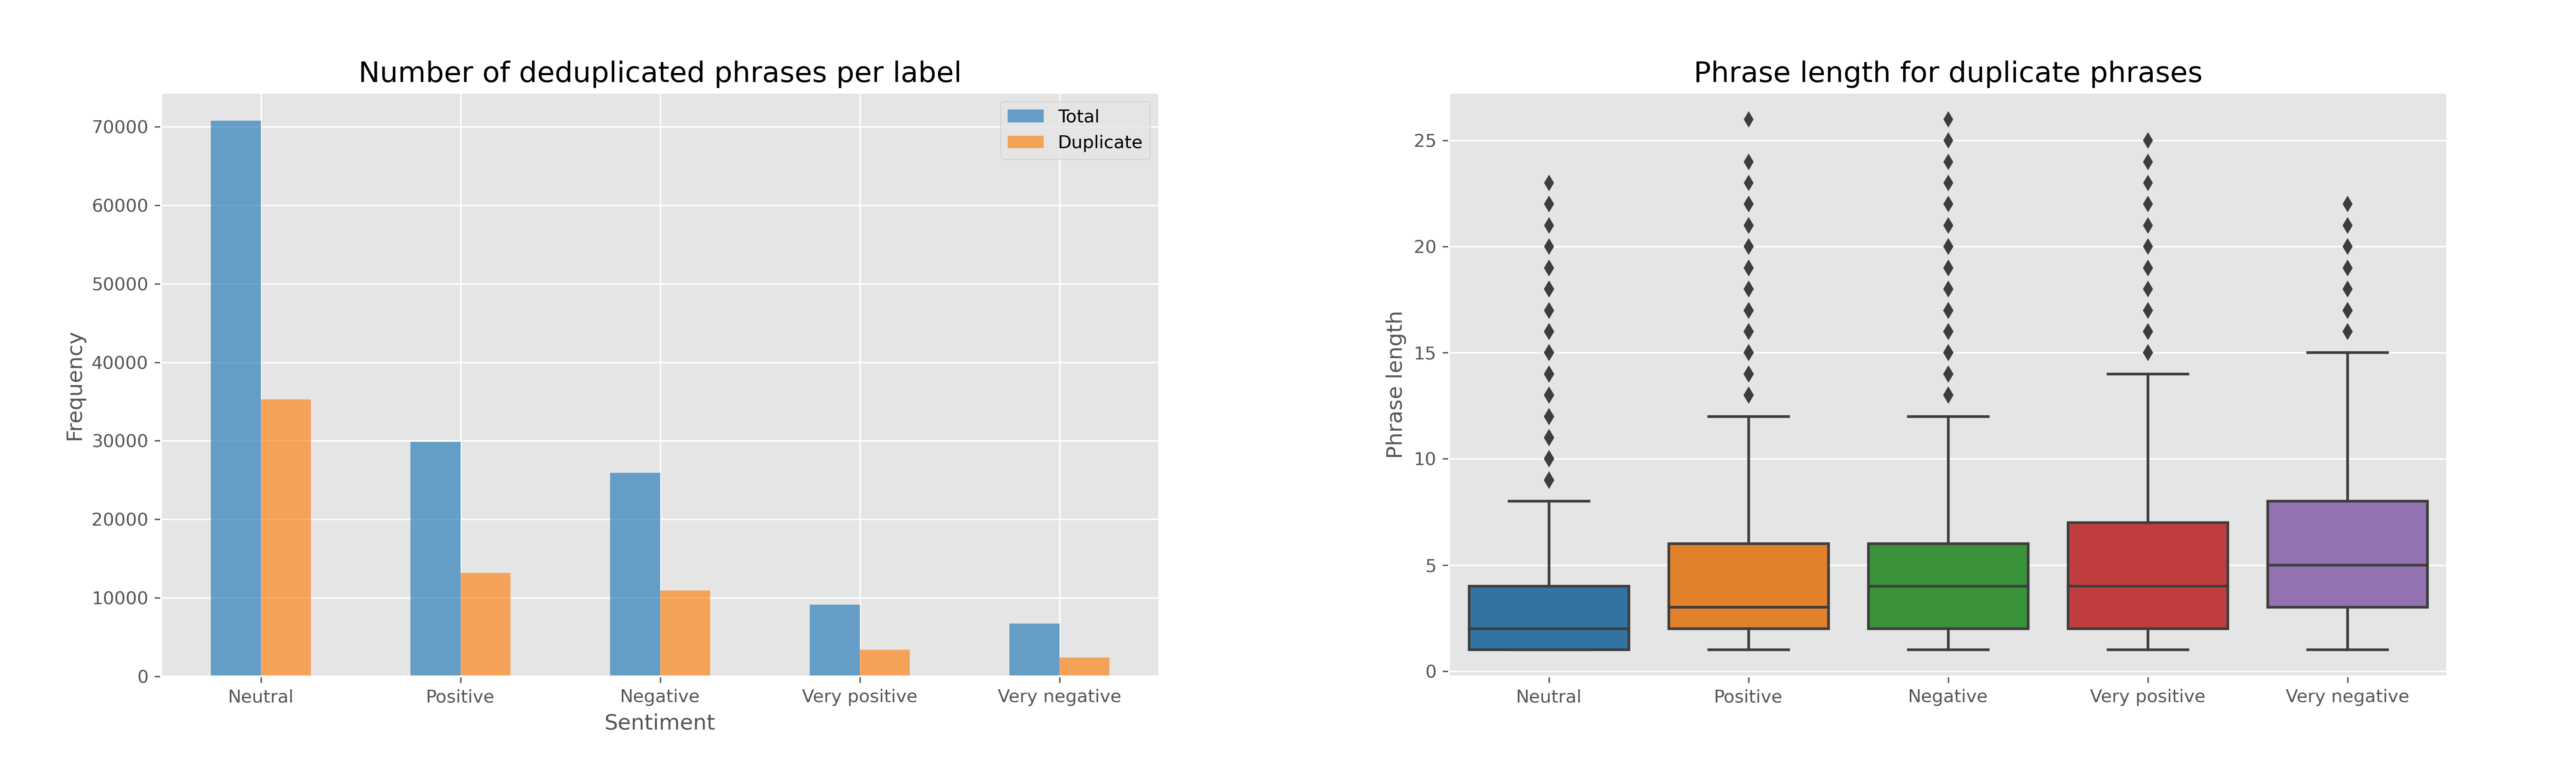
\includegraphics[width=1.0\textwidth]{DME-template/duplicates.png}
    \caption{Number of duplicate phrases per sentiment category, and boxplot showing the word count of duplicate phrases for each sentiment class.}
    \label{fig:class-balance}
\end{figure} 

\subsection{Feature Engineering}

Considering that the dataset is imbalanced, it's difficult to discriminate positive and negative observations from neutral ones. Due to this, we would like to include additional features which may increase the predictive power of our selected supervised algorithms. The authors \cite{socher-etal-2013-recursive} state that stronger sentiment builds up in longer phrases, whereas the majority of shorter phrases are neutral. Therefore, including word count as an additional feature may be valuable in discriminating the extreme sentiments from neutral sentiment. Figure \ref{fig:kde} shows a kernel density plot of phrase length for each sentiment label. We can see that for each category the distribution is heavily left skewed. However, the probability mass is slightly more concentrated in the right tails of the extreme sentiments than it is for neutral sentiment. This further indicates that longer phrases are more frequent with emotional text. 

\begin{figure}[h]
    \centering
    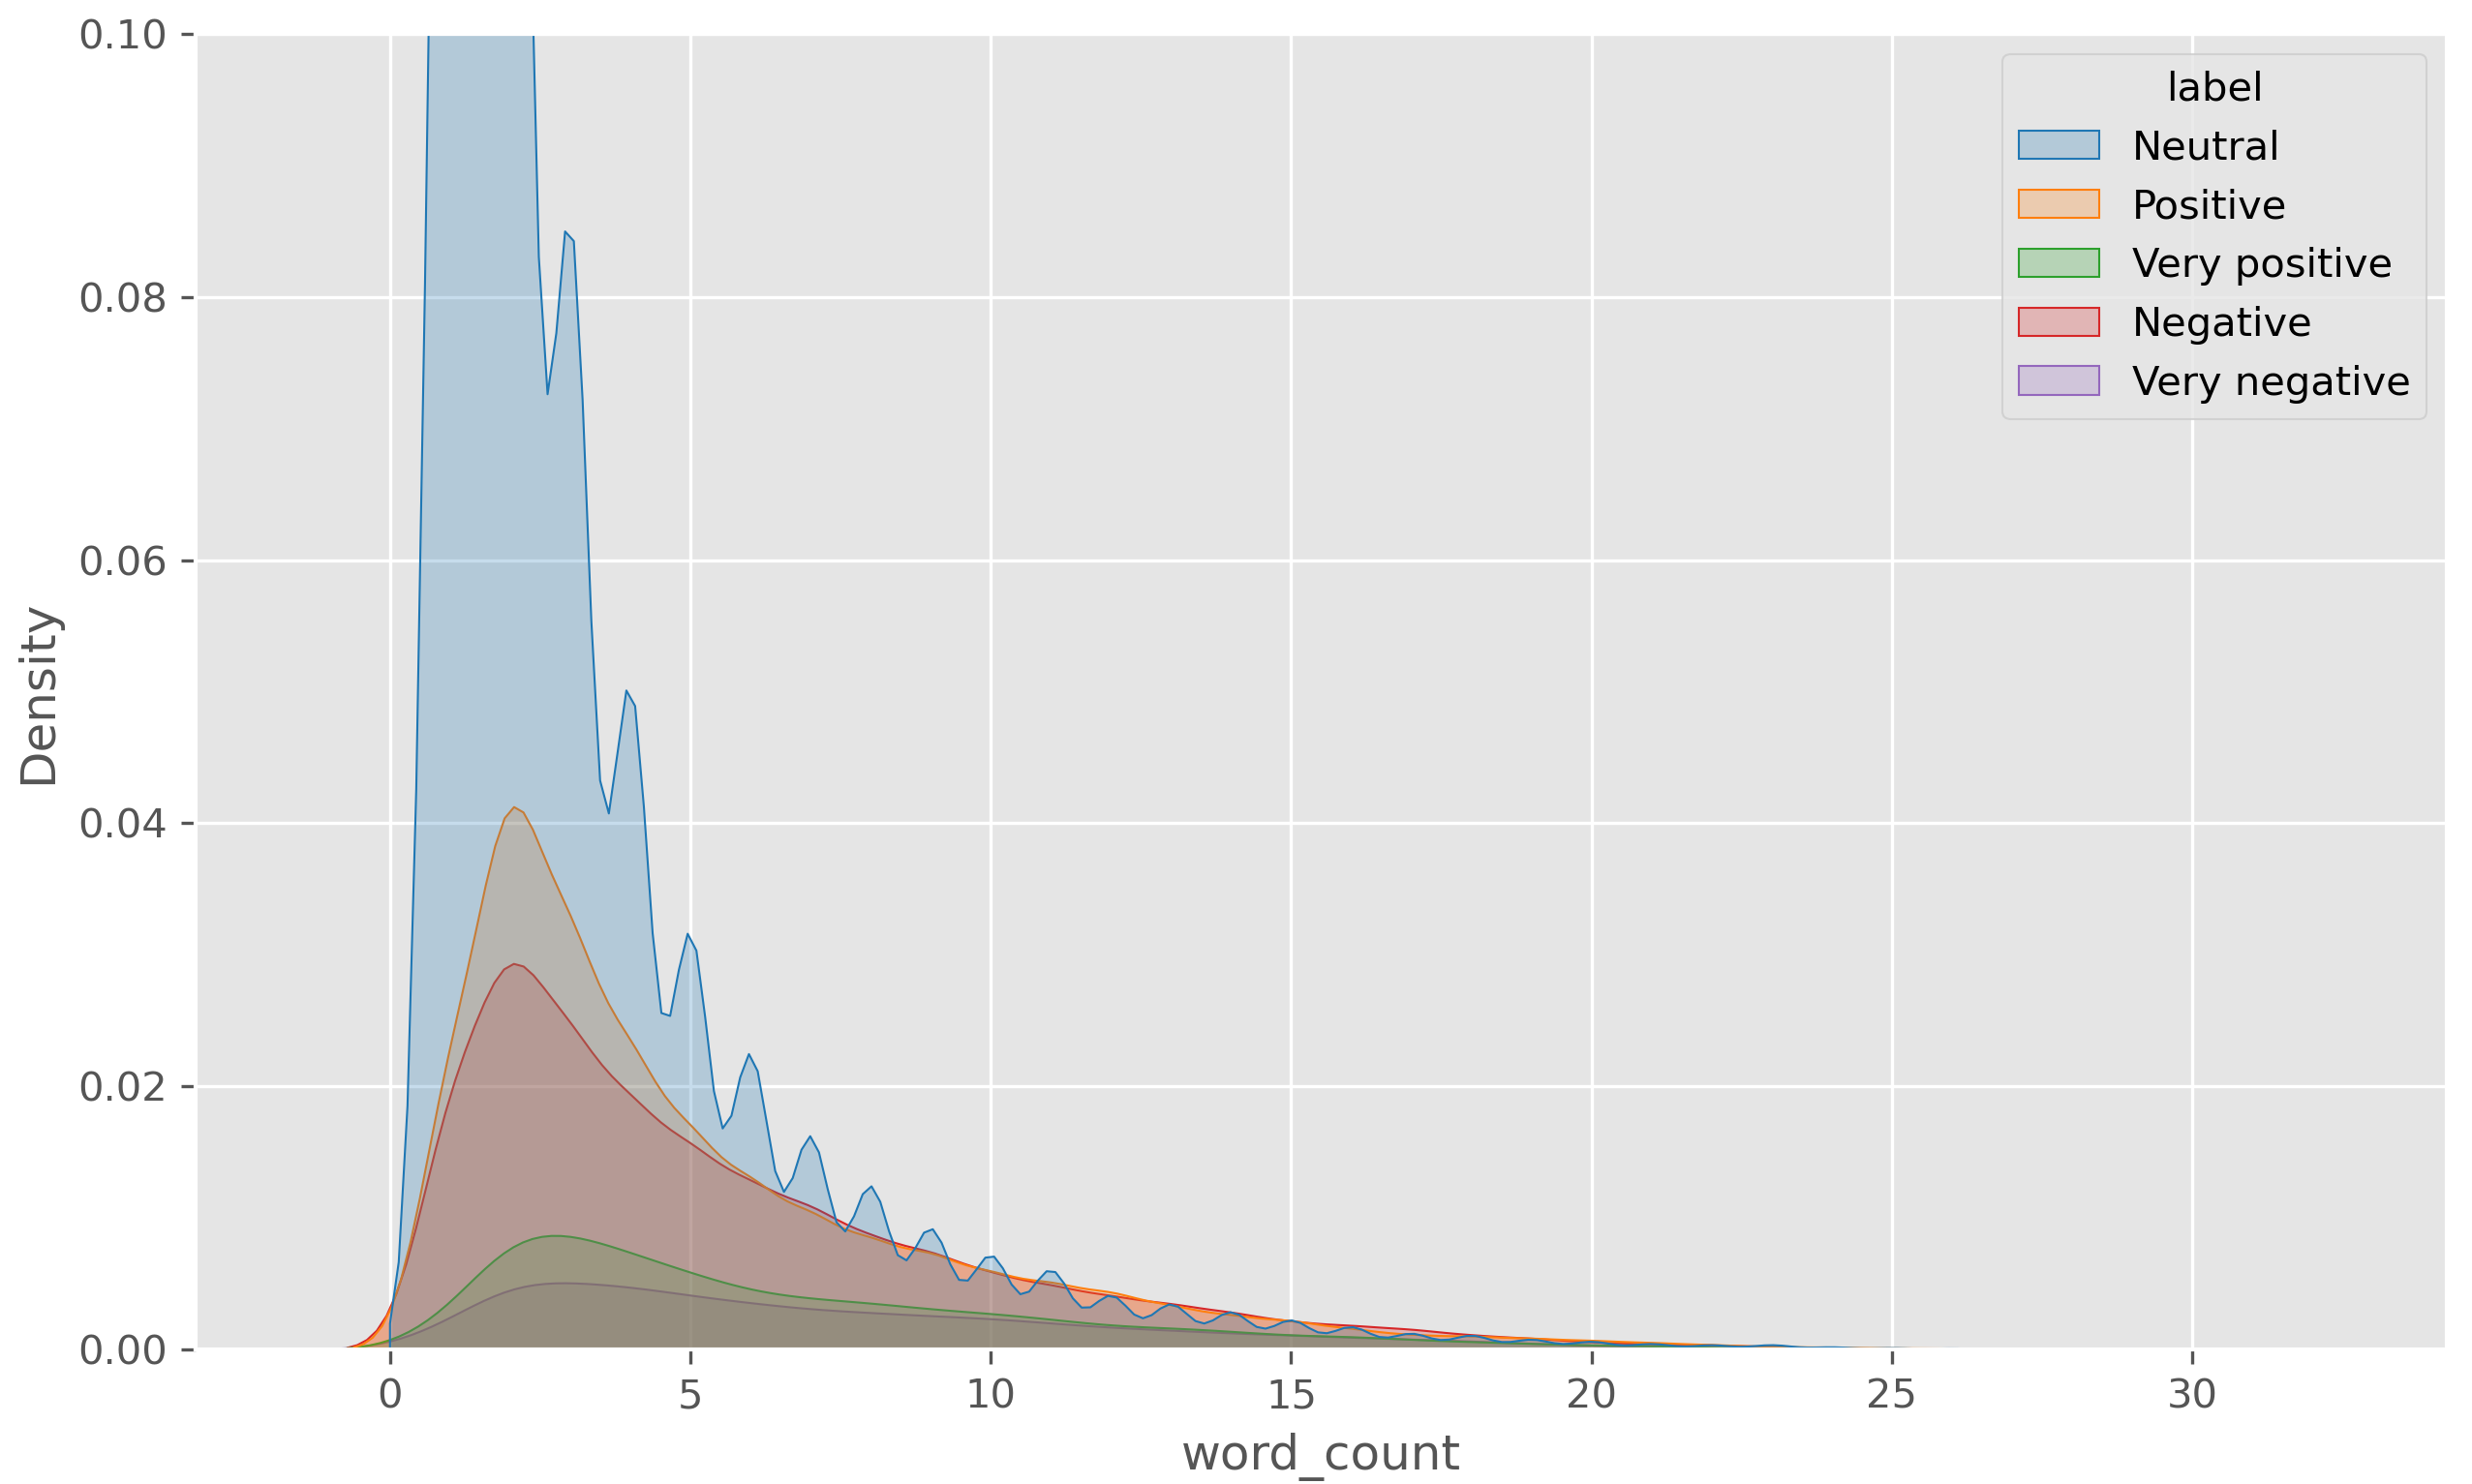
\includegraphics[width=0.75\textwidth]{DME-template/kde_cropped.png}
    \caption{Kernel density plots showing the distribution of phrase length for each sentiment class. Note that the y-axis has been clipped to make the graph more interpretable.}
    \label{fig:kde}
\end{figure}

\subsection{Dimensionality Reduction}
Figure \ref{fig:lda} displays the input data projected to two dimensions using LDA. While there is some overlap between data points, we see that predominantly LDA does an excellent job in separating each sentiment category into their own distinct regions in space. Additionally, the right-hand-side image of Figure \ref{fig:lda} shows us that approximately all of the TF-IDF input vector variance can be captured by the first four components.  

\begin{figure}[h]
    \setlength{\belowcaptionskip}{-10pt}
    \centering
    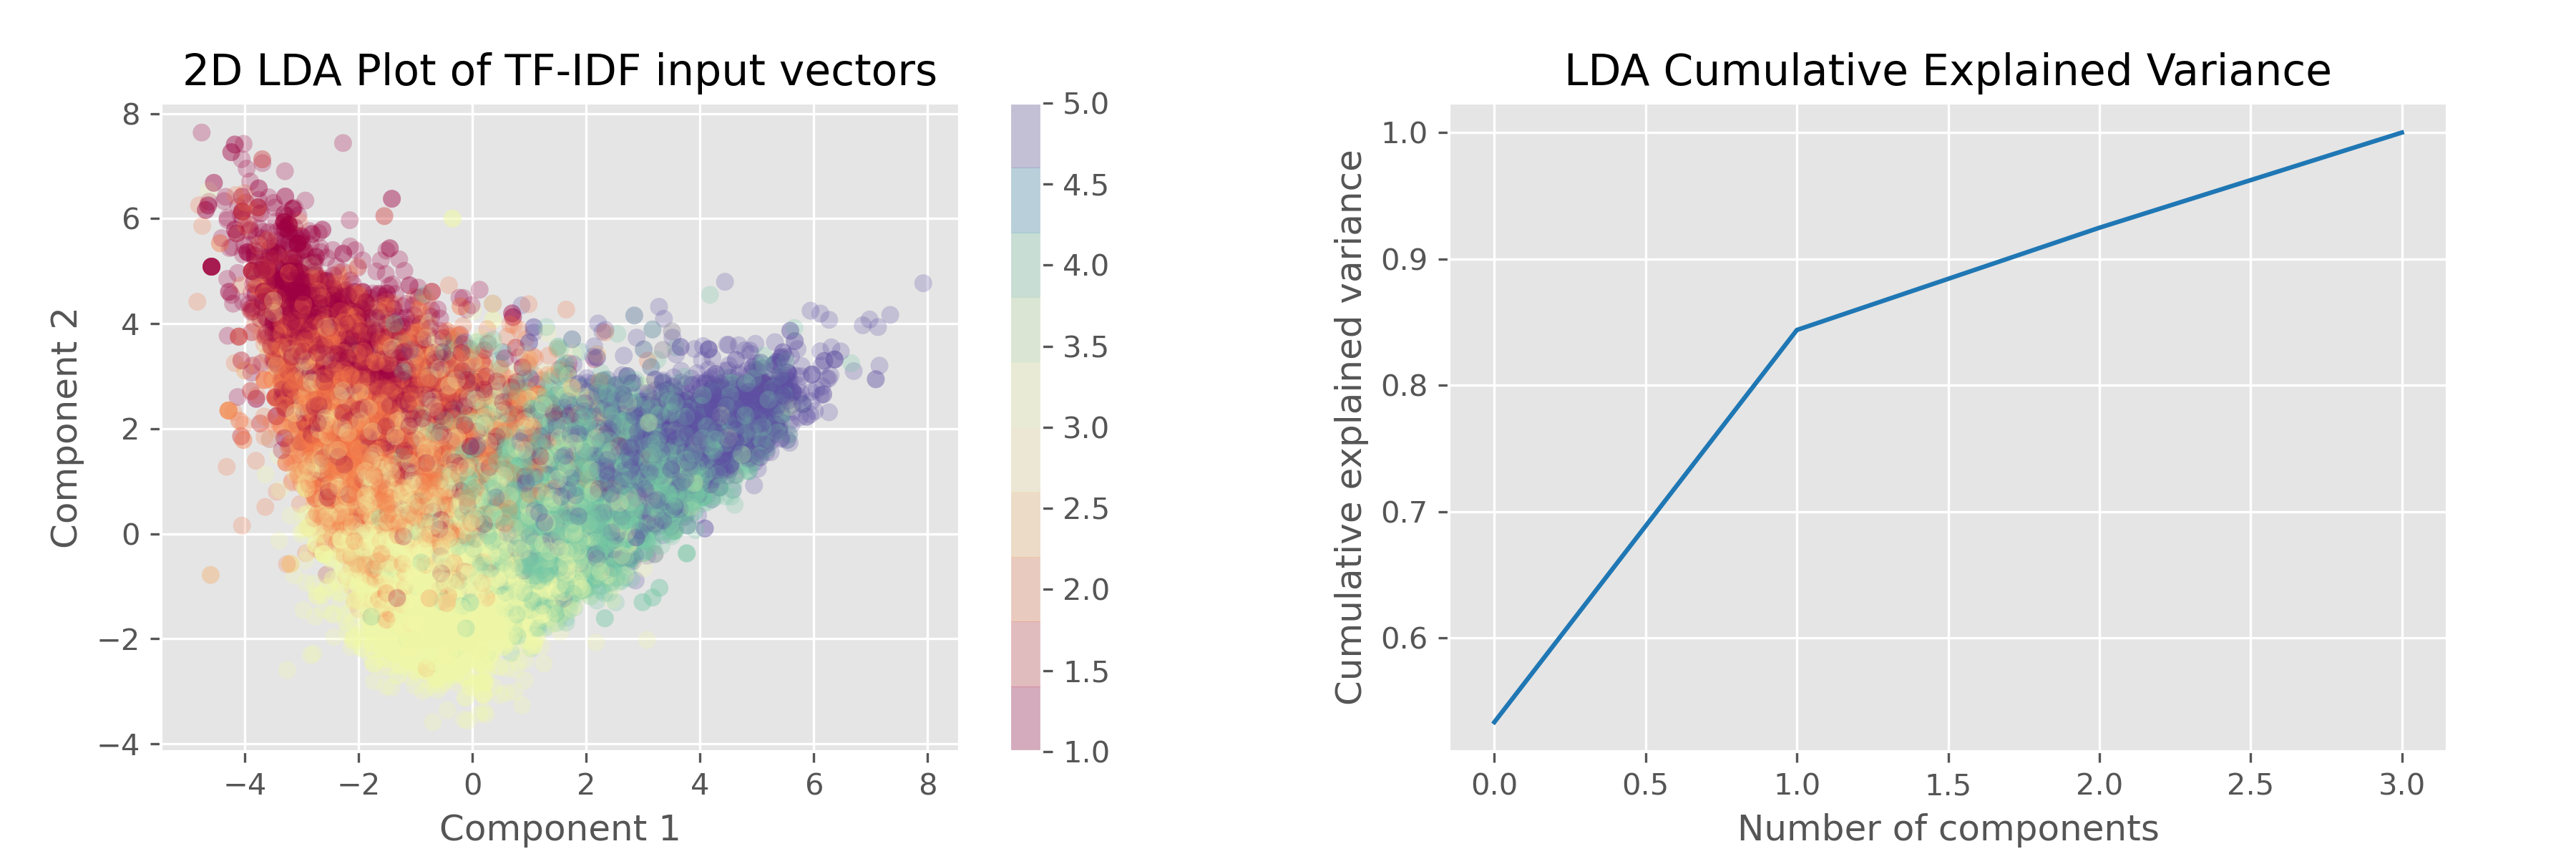
\includegraphics[width=1.0\textwidth]{DME-template/lda.png}
    \caption{Left: TF-IDF input vectors projected to 2D using LDA. \textit{1 - Very Negative, 2 - Negative, 3 - Neutral, 4 - Positive}, and \textit{5 - Very positive.} Right: Cumulative explained variance ratio as a function of the number of components.}. 
    \label{fig:lda}
\end{figure}

\section{Supervised Learning}
\label{SL}

\subsection{Learning Methods}

To estimate generalisation performance, we employ a two times hold-out approach such that the dataset $D$ is split into training $D^{train}$, validation $D^{val}$ and testing $D^{test}$ subsets using a split ratio of 60/20/20. As described in Section \ref{data-prep}, prior to training and evaluation, we convert the phrases into TF-IDF feature vectors. Based on the insights gained from exploratory data analysis, we include phrase length as an additional feature, and reduce the dimensionality of the feature vectors using LDA. Performance is evaluated against $D^{val}$ using a variety of classification models provided by the Sklearn library.\footnote{\url{https://scikit-learn.org/stable/}} The models and hyperparameters used are listed in Table \ref{tab:class-models} in the appendix. The dummy classifier is selected to act as a baseline, whereas subsequent classifiers are selected based on increasing complexity. With Gaussian Naive Bayes, Logistic Regression and the Linear SVM being more simplistic linear models, and the RBF SVM, Random Forest, and MLP being more complicated non-linear methods, we're interested in observing whether there is a correlation between model complexity and better performance.

We evaluate performance on $D^{val}$ using accuracy, macro-precision, macro-recall, macro-f1, and Cohen's kappa. Results based on accuracy should be taken with a grain of salt due to the dataset imbalance. Thus, the best performing model is selected based on performance on the remaining metrics. Using the best performing model, we re-estimate its parameters on the union of the training and validation data $D^{train} \cup D^{val}$ as this allows us to estimate the prediction model more accurately. Finally, we take $D^{test}$ and compute an estimate of the prediction loss using the best performing model fitted on $D^{train} \cup D^{val}$.

Note that for precision, recall, and F1 score, we use the macro-variant as we are interested in assessing how the models perform overall across the entire dataset. Additionally, we use Cohen's Kappa as it is more informative when working with imbalanced data. 

\subsection{Results}

Table \ref{tab:feat-class-eval} summarises the results obtained on the validation set using the aforementioned additional features. We see that all classifiers perform better than the selected baseline dummy classifier. While the random forest classifier achieves the highest macro-precision score, we can see that across the remaining meaningful metrics, the MLP achieves the best performance. In particular, the model achieves a macro-recall of 49.8\%, macro-f1 of 51.6\% and a Kappa score of 42.2\%. Although the results aren't exceptional, this is to be expected considering the challenges associated with the task. Regarding model complexity, we see that the more complicated non-linear methods perform better across the majority of metrics. 

\begin{table*}[h]
\caption{Evaluation of classifiers on validation set.} 
\label{tab:feat-class-eval}
\centering 
\setlength\aboverulesep{0pt}
\setlength\belowrulesep{0pt}
\setlength\doublerulesep{0pt}
\setlength\extrarowheight{3pt}
\small
\begin{tabularx}{0.9\textwidth}{l p{1.5cm} XXXXX}
    \toprule
    Model & Accuracy & Precision & Recall & F1 & Kappa \\
    \midrule 
    DummyClassifier (Most Frequent) & 0.498 & 0.100 & 0.200 & 0.133 & 0.000 \\ 
    Gaussian Naive Bayes & 0.611 & 0.521 & 0.500 & 0.509 & 0.404 \\ 
    Logistic Regression & 0.622 & 0.554 & 0.469 & 0.499 & 0.405 \\ 
    Linear SVM & 0.606 & 0.540 & 0.432 & 0.442 & 0.401 \\ 
    RBF SVM & \textbf{0.627} & 0.559 & 0.463 & 0.493 & 0.413 \\ 
    Random Forest & \textbf{0.627} & \textbf{0.549} & 0.493 & 0.515 & 0.421 \\ 
    \textbf{MLP} & 0.624 & 0.540 & \textbf{0.498} & \textbf{0.516} & \textbf{0.422} \\ 
    \bottomrule
\end{tabularx}
\end{table*}

To assess whether or not including phrase length as an additional feature has any discriminatory impact, we also evaluate performance on the validation set without it. Table \ref{tab:class-eval} summarises the results, where improvements in model performance are colored in green and worse performance is colored in red. While we see that some models attain no benefit or harm from including phrase length as an additional feature, a few models perform worse. For example, we can see that performance decreased in terms of all metrics despite macro-precision for the MLP. Although the changes in performance are minimal, the decrease in validation performance for numerous models could suggest that phrase length has some importance for the classification task.

By comparing the performance of multiple classifiers on $D^{val}$, our results are only an approximation of the generalisation error on unseen data. Nonetheless, we believe this is a fairly accurate estimate considering the size of $D^{val}$ (45,449 observations).

\begin{table*}[h]
\caption{Evaluation of classifiers on validation set without phrase length as an additional feature. Improvements in model performance are colored in green, and worse performance is colored in red.} 
\label{tab:class-eval}
\centering 
\setlength\aboverulesep{0pt}
\setlength\belowrulesep{0pt}
\setlength\doublerulesep{0pt}
\setlength\extrarowheight{3pt}
\small
\begin{tabularx}{0.9\textwidth}{l p{1.5cm} XXXXX}
    \toprule
    Model & Accuracy & Precision & Recall & F1 & Kappa \\
    \midrule 
    DummyClassifier (Most Frequent) & 0.498 & 0.100 & 0.200 & 0.133 & 0.000 \\ 
    Gaussian Naive Bayes & 0.611 & 0.521 & 0.500 & 0.509 & 0.404 \\ 
    Logistic Regression & 0.622 & \cellcolor{red!25}0.553 & 0.469 & \cellcolor{red!25}0.498 & 0.405 \\ 
    Linear SVM & \cellcolor{green!25}0.609 & \cellcolor{red!25}0.535 & \cellcolor{red!25}0.425 & \cellcolor{green!25}0.450 & \cellcolor{red!25}0.375 \\ 
    RBF SVM & 0.627 & 0.559 & 0.463 & 0.493 & 0.413 \\ 
    Random Forest & 0.627 & \cellcolor{red!25}0.548 & \cellcolor{red!25}0.492 & \cellcolor{red!25}0.514 & \cellcolor{green!25}0.422 \\ 
    MLP & \cellcolor{red!25}0.623 & \cellcolor{green!25}0.546 & \cellcolor{red!25}0.483 & \cellcolor{red!25}0.506 & \cellcolor{red!25}0.418 \\
    \bottomrule
\end{tabularx}
\end{table*}

We fit the top two performing models from Table \ref{tab:feat-class-eval} on $D^{train} \cup D^{val}$ and observe their performance on $D^{test}$. The results are presented in Table \ref{tab:test-res}. We see that both models achieve better performance across all the selected evaluation metrics except macro-recall which decreased from 49.8\% to 49.2\% for the MLP. By re-estimating the model's parameters on the union of the training and validation data, it's likely that the improved performance is due to an increase in data. 

\begin{table*}[h]
\caption{Best performing model results on test set.} 
\label{tab:test-res}
\centering 
\setlength\aboverulesep{0pt}
\setlength\belowrulesep{0pt}
\setlength\doublerulesep{0pt}
\setlength\extrarowheight{3pt}
\small
\begin{tabularx}{0.9\textwidth}{XXXXXX}
    \toprule
    Model & Accuracy & Precision & Recall & F1 & Kappa \\
    \midrule 
    Random Forest & 0.635 & 0.573 & 0.500 & 0.528 & 0.434 \\ 
    MLP & 0.628 & 0.565 & 0.492 & 0.518 & 0.429 \\ 
    \bottomrule
\end{tabularx}
\end{table*}

\section{Unsupervised Learning}

\subsection{Learning Methods}

In this section we employ unsupervised non-linear dimensionality reduction algorithms to compress the data and unsupervised clustering algorithms for classification. Algorithms in this section use TF-IDF vector representations of the dataset phrases while considering the top 2,000 words ordered by term frequency. Identical train, validation and test dataset splits are being used as in Section \ref{SL}. 

For dimensionality reduction two approaches are tested: (1) fully-connected auto-encoders trained by reconstructing TF-IDF vectors with various sizes of bottleneck hidden layers, chosen due to being practically simple parametric models with great performance, and (2) reduction using the UMAP \cite{mcinnes2018umap} algorithm, chosen due to being the state-of-the-art in non-parametric dimensionality reduction. Our goal is to inspect the performance differences during the clustering phase between the parametric and non-parametric approaches, and between the embedding vectors and original TF-IDF vectors. Although linear approaches such as SVD and Principal Component Analysis were attempted, these were not reported due to poor compression performance on the sparse TF-IDF vectors.

For clustering, three unsupervised clustering approaches are selected: (1) k-means, selected due to its simplicity and quick computation, (2) Spectral Clustering, selected due to being considered as an improvement of k-means, and (3) Agglomerative Clustering, due to anticipated high clustering performance. Similar to supervised learning, we attempt to classify the phrase data into 5 classes, therefore, for each clustering algorithm we form 5 clusters. 

In order to determine meaningful categories for the formed clusters, we make use of a small amount of labels from $D^{val}$. The retrieved cluster numbers are mapped to these labels to attain the highest label overlap. For the sake of simplicity and practicality, we select 200 labeled validation set examples for comparison. This label mapping is further used to assess performance against $D^{test}$. Similar to the approach taken in Section \ref{SL}, we assess performance using macro-precision, macro-recall, macro-f1, and Cohen's Kappa. We ignore accuracy due to a heavy imbalance in the number of samples assigned to each cluster. Nonetheless, for comparison with our supervised methods, accuracy values are provided by Figure \ref{fig:usl-acc} in the appendix. 

\subsection{Results}

As can be seen by Figure \ref{fig:metrics}, the performance of Agglomerative Clustering using embedding vectors generated by an auto-encoder proves best on average across all evaluation metrics. UMAP embeddings took substantially longer to compute compared to the auto-encoder approach, making the fully-connected auto-encoder a favourable approach. However, both dimensionality reduction algorithms provide a noticeable clustering performance improvement in comparison to the original TF-IDF vectors. 

Figure \ref{fig:cluster-bases} displays the dimensions of the embedding vectors of size 2 and the respective labels. The distribution of samples and their labels display no clear separation, therefore the assignment of clusters is not trivial. In cases where many samples are crammed in one space and some of them are scattered, one cluster usually gets assigned to a large bunch of various labels (as shown by the UMAP example in Figure \ref{fig:cluster-bases}), therefore assigning one specific label to the majority of input samples during inference. These tendencies extend to some extent to higher-dimensional embeddings and other clustering algorithms.

\section{Conclusions}

In this report we used the SST dataset to tackle the task of fine-grained phrase-level sentiment analysis using both supervised and unsupervised methods. For supervised learning, we explored the use of LCA as a dimensionality reduction method on TF-IDF feature vectors, and we explored including word frequency as an additional feature to increase the predictive power of our selected classifiers.  

Using a two-times hold out approach for evaluation, our supervised classification results showed that the best performing model on the held-out test set was the Random Forest classifier, achieving a Macro-F1 of 52.8\% and a Kappa score of 43.4\%. Additionally, we found that including phrase length appears to have some importance in improving performance on the classification task. Performance could likely be further improved by hyperparameter tuning and cross validation, and by more extensive feature engineering related to part of speech tags, term positions and negation. 

With regards to unsupervised learning, the results were considerably worse in comparison to the supervised approach, however, this comes at no surprise considering the challenges associated with clustering very high dimensional data. Nonetheless, we explored k-means, Spectral Clustering, and Agglomerative Clustering on dimensionality reduced TF-IDF feature vectors produced by a fully-connected auto-encoder and UMAP. We found the performance of Agglomerative Clustering using embeddings produced by the fully-connected auto-encoder to achieve the best results on the vast majority of evaluation metrics. 

\begin{figure}[h]
    \centering
    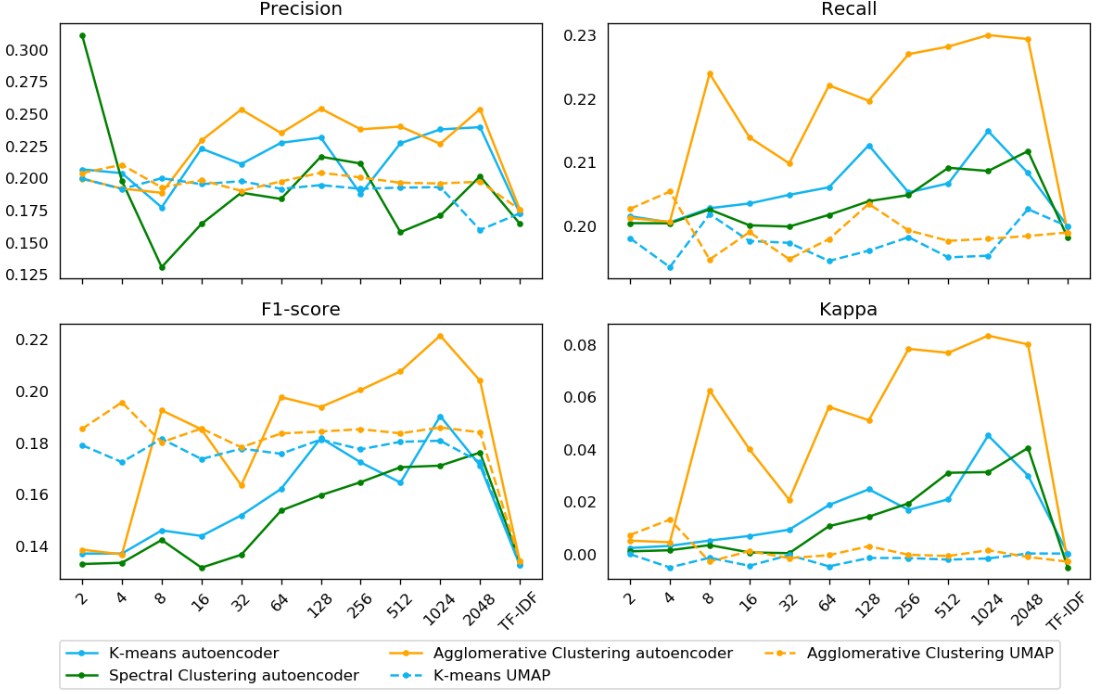
\includegraphics[width=1.0\textwidth]{DME-template/metrics.png}
    \caption{Performance of tested algorithms. X axis marks the length of embedding vectors or whether these vectors are the original TF-IDF vectors. Y axis marks metric value. Lines and related legend depicts what kind of clustering algorithm and dimensionality reduction approach was used. }
    \label{fig:metrics}
\end{figure}

\begin{figure}[h]
    \centering
    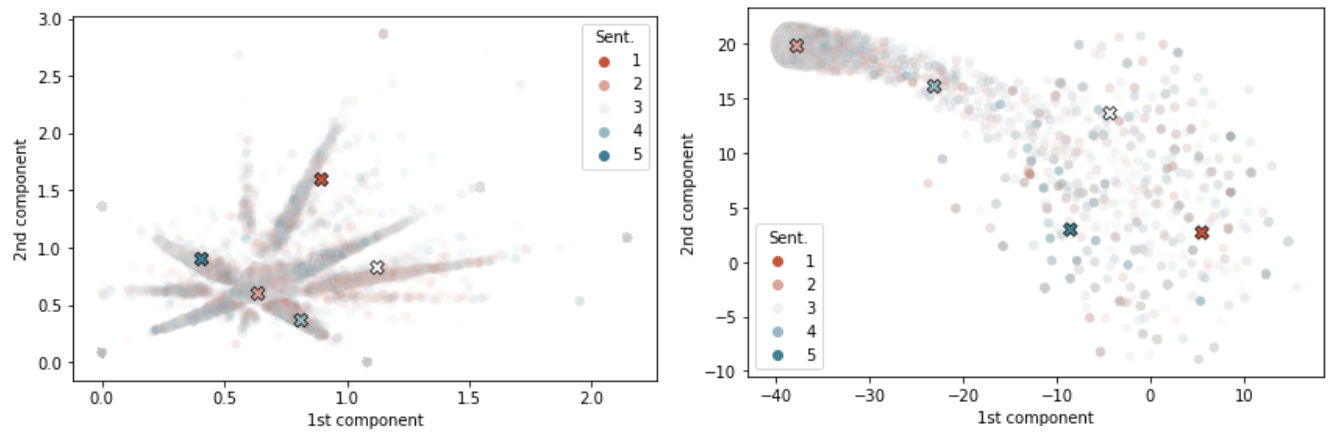
\includegraphics[width=1.0\textwidth]{DME-template/cluster_bases.png}
    \caption{Distribution of training labels in embedding dimensions for vectors of size 2 for auto-encoder embeddings (left) and UMAP (right). Both x and y axes mark the respective components of the embedding vector. The legend maps the colour to sentiment label. "o" labels show the training examples in embedding dimensions and "x" labels show clustering bases assigned by k-means. }
    \label{fig:cluster-bases}
\end{figure}

\newpage
\bibliographystyle{IEEEtranS}

\bibliography{main}

\section*{Statement of Contribution}

The work for this report was managed equally by both group members. We split the provided tasks among us such that Oliver primarily implemented the supervised methods, and exploratory data analysis whilst Dainius implemented unsupervised learning techniques, and conducted research on relevant background and previous work. We both communicated via Microsoft Teams, and shared code between each other using a private GitHub repository.

\section*{Appendix}

\begin{table*}[h]
\caption{Classification models.} 
\label{tab:class-models}
\centering 

\begin{tabularx}{1.0\textwidth}{l p{9.0cm} X}
    \toprule
    Model & Hyperparameters \\
    \midrule 
    Dummy Classifier (Baseline) & \emph{Most frequent} strategy, which simply predicts the most \\ & frequent label in the training set. \\ 
    Gaussian Naive Bayes & . \\
    Logistic Regression & L2 Regularisation, and 10,000 training iterations. \\ 
    Support Vector Machine & Linear kernel, squared hinge loss, and 1000 training \\
    & iterations. \\ 
    Support Vector Machine & Radial Basis Function kernel. \\ 
    Random Forest & 50 trees, and a maximum depth of 10 leaves. \\ 
    Multi-layer Perceptron & One hidden layer of size 100, ReLU activation function, \\ 
    & a learning rate of 0.0001 with Adam optimisation. \\
    \bottomrule
\end{tabularx}
\end{table*}

\begin{figure}[p]
    \centering
    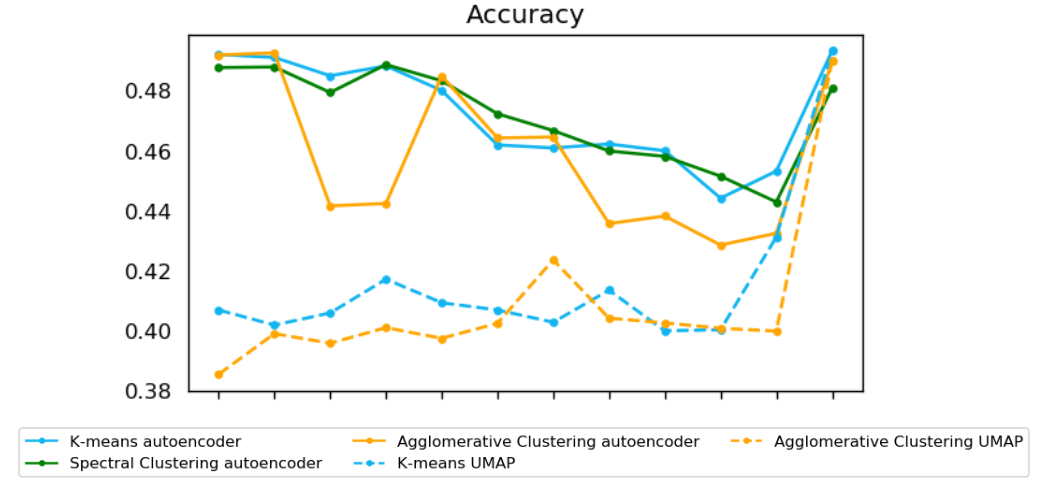
\includegraphics[width=1.0\textwidth]{DME-template/Accuracy.png}
    \caption{Accuracy metric of tested unsupervised algorithms. X axis marks the length of embedding vectors or whether these vectors are original TF-IDF vectors. Y axis marks metric value. Lines and related legend depicts what kind of clustering algorithm and dim. reduction approach was used. }
    \label{fig:usl-acc}
    \vspace{128in}
\end{figure}

\end{document}
